\begin{figure}[htbp]
    \centering
    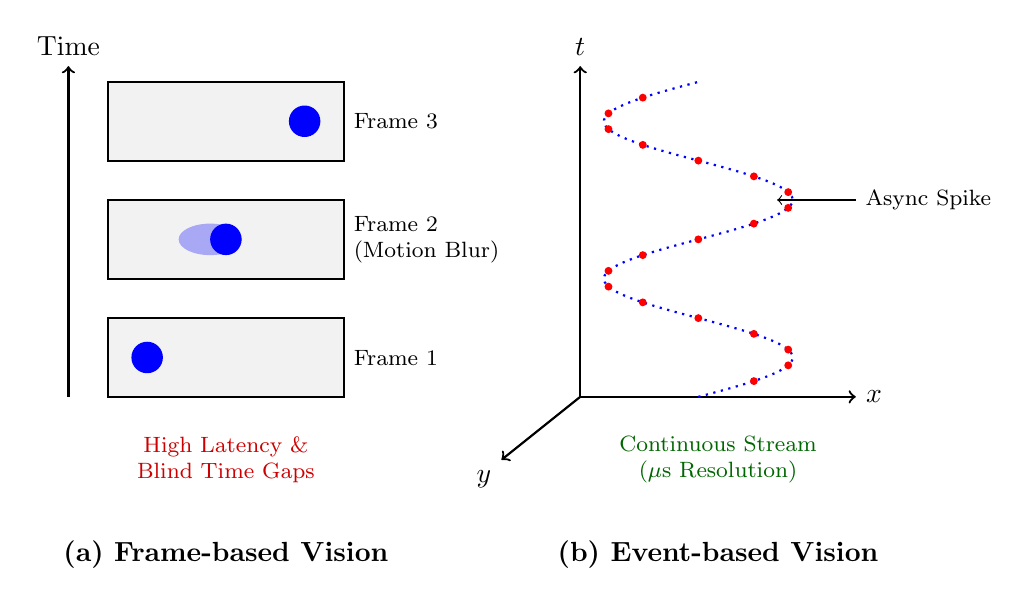
\begin{tikzpicture}
        % ================= 左图：Frame-based =================
        \begin{scope}[shift={(-3.5,0)}]
            % 1. 画时间轴箭头
            \draw[->, thick] (-0.5, 0) -- (-0.5, 4.2) node[above] {Time};
            
            % 2. Frame 1 (t=0)
            \draw[thick, fill=gray!10] (0, 0) rectangle (3, 1);
            \fill[blue] (0.5, 0.5) circle (0.2); 
            \node[right, font=\footnotesize] at (3, 0.5) {Frame 1};
            
            % 3. Frame 2 (t=1) - 模拟运动模糊
            \draw[thick, fill=gray!10] (0, 1.5) rectangle (3, 2.5);
            \fill[blue, opacity=0.3] (1.3, 2.0) ellipse (0.4 and 0.2); 
            \fill[blue] (1.5, 2.0) circle (0.2); 
            \node[right, font=\footnotesize, align=left] at (3, 2.0) {Frame 2\\(Motion Blur)};
            
            % 4. Frame 3 (t=2)
            \draw[thick, fill=gray!10] (0, 3.0) rectangle (3, 4.0);
            \fill[blue] (2.5, 3.5) circle (0.2); 
            \node[right, font=\footnotesize] at (3, 3.5) {Frame 3};
            
            % 5. 缺点描述 (红色文字)
            \node[red!80!black, font=\footnotesize, align=center] at (1.5, -0.8) {High Latency \&\\Blind Time Gaps};

            % 6. 【修改位置】标题移动到底部
            \node[font=\bfseries] at (1.5, -2.0) {(a) Frame-based Vision};
        \end{scope}

        % ================= 右图：Event-based =================
        \begin{scope}[shift={(2.5,0)}]
            % 1. 画 3D 坐标轴 (x, y, t)
            \draw[->, thick] (0,0) -- (3.5,0) node[right] {$x$};
            \draw[->, thick] (0,0) -- (0,4.2) node[above] {$t$};
            \draw[->, thick] (0,0) -- (-1,-0.8) node[below left] {$y$};
            
            % 2. 画螺旋轨迹 (Spikes)
            \draw[blue, thick, dotted] plot[domain=0:4, samples=100] ({1.5 + 1.2*sin(180*\x)}, \x);
            
            % 3. 添加脉冲点 (Spikes)
            \foreach \t in {0.2, 0.4, ..., 3.8} {
                \fill[red] ({1.5 + 1.2*sin(180*\t)}, \t) circle (0.05);
            }
            
            % 4. 优势描述 (绿色文字)
            \node[green!40!black, font=\footnotesize, align=center] at (1.75, -0.8) {Continuous Stream\\($\mu$s Resolution)};
            
            % 5. 标注 Spike Event
            \draw[<-, thin] (2.5, 2.5) -- (3.5, 2.5) node[right, font=\footnotesize] {Async Spike};

            % 6. 【修改位置】标题移动到底部
            \node[font=\bfseries] at (1.75, -2.0) {(b) Event-based Vision};
        \end{scope}

    \end{tikzpicture}
    
    \caption{Visual comparison of acquisition paradigms. \textbf{(a)} Standard frame-based 
    cameras capture discrete snapshots with fixed intervals, suffering from blind spots between
     frames and motion blur. \textbf{(b)} Event-based sensors 
     record asynchronous spikes with microsecond resolution, forming a continuous trajectory in 
     space-time ideal for high-speed control.}
    \label{fig:frame_vs_event}
\end{figure}